% ARKHEION AGI 2.0 - Paper 36: Trading Intelligence
% Jhonatan Vieira Feitosa | Manaus, Amazonas, Brazil
% February 2026

\documentclass[11pt,twocolumn]{article}

% Encoding and fonts
\usepackage[utf8]{inputenc}
\usepackage[T1]{fontenc}
\usepackage{lmodern}

% Layout
\usepackage[margin=0.75in]{geometry}
\usepackage{fancyhdr}

% Mathematics
\usepackage{amsmath,amssymb}

% Graphics and colors
\usepackage{xcolor}
\usepackage{tikz}
\usetikzlibrary{arrows.meta,shapes,positioning}

% Tables
\usepackage{booktabs}

% Code listings
\usepackage{listings}

% Hyperlinks
\usepackage{hyperref}

% ==================== COLORS ====================
\definecolor{arkblue}{RGB}{0,102,204}
\definecolor{arkpurple}{RGB}{102,51,153}
\definecolor{arkgreen}{RGB}{0,153,76}
\definecolor{arkgold}{RGB}{218,165,32}

% ==================== LISTINGS ====================
\lstset{
    basicstyle=\ttfamily\scriptsize,
    breaklines=true,
    breakatwhitespace=true,
    postbreak=\mbox{\textcolor{gray}{$\hookrightarrow$}\space},
    columns=flexible,
    keepspaces=true,
    showstringspaces=false,
    numbers=none,
    backgroundcolor=\color{gray!5},
    frame=single,
    rulecolor=\color{gray!30}
}

% ==================== HEADER/FOOTER ====================
\pagestyle{fancy}
\fancyhf{}
\fancyhead[L]{\small\textcolor{arkblue}{ARKHEION AGI 2.0}}
\fancyhead[R]{\small Paper 36: Trading Intelligence}
\fancyfoot[C]{\thepage}
\renewcommand{\headrulewidth}{0.4pt}

% ==================== HYPERREF ====================
\hypersetup{
    colorlinks=true,
    linkcolor=arkblue,
    urlcolor=arkpurple,
    citecolor=arkgreen
}

% ==================== TITLE ====================
\title{
    \vspace{-1.5cm}
    {\Large\textbf{Trading Intelligence}}\\[0.3em]
    {\large $\phi$-Enhanced Financial Reasoning}\\[0.2em]
    {\normalsize ARKHEION AGI 2.0 --- Paper 36}
}

\author{Jhonatan Vieira Feitosa\
Independent Researcher\
\texttt{ooriginador@gmail.com}\
Manaus, Amazonas, Brazil}

\date{February 2026}

\begin{document}

\maketitle

% ==================== ABSTRACT ====================
\begin{abstract}
\noindent
This paper presents \textbf{Trading Intelligence}, a financial analysis and portfolio optimization module for ARKHEION AGI 2.0. The system combines \textbf{technical analysis}, \textbf{$\phi$-enhanced optimization}, and \textbf{risk management} to support investment decisions. This is a \textbf{research prototype}---not financial advice. The architecture demonstrates how AGI capabilities can be applied to financial domains while maintaining transparency and risk awareness.

\vspace{0.5em}
\noindent\textbf{Keywords:} algorithmic trading, portfolio optimization, risk management, Fibonacci, financial AI

\vspace{0.5em}
\textbf{Disclaimer:} This paper describes research software. No financial advice is provided. Past performance does not guarantee future results. Cryptocurrency and securities trading involves substantial risk of loss.
\end{abstract}

% ==================== EPISTEMOLOGICAL NOTE ====================
\section*{Epistemological Note}
\textit{This paper is \textbf{primarily heuristic}. Financial markets are complex adaptive systems where backtesting rarely predicts future performance:}

\begin{center}
\footnotesize
\begin{tabular}{@{}ll@{}}
\toprule
\textbf{Heuristic} & \textbf{Status} \\
\midrule
``$\phi$ optimization'' & Research exploration \\
``Fibonacci levels'' & Technical analysis tool \\
``Portfolio optimization'' & Markowitz framework \\
\bottomrule
\end{tabular}
\end{center}

\textbf{Warning:} No backtested results are presented as predictive of future returns.

% ==================== INTRODUCTION ====================
\section{Introduction}

Financial markets present unique challenges for AI:
\begin{itemize}
    \item \textbf{Non-stationarity}: Patterns change over time
    \item \textbf{Reflexivity}: Predictions affect outcomes
    \item \textbf{Noise}: Signal-to-noise is low
    \item \textbf{Risk}: Substantial losses possible
\end{itemize}

ARKHEION's Trading Intelligence explores how AGI capabilities can assist (not replace) human financial decision-making.

% ==================== TECHNICAL ANALYSIS ====================
\section{Technical Analysis}

\subsection{Fibonacci Levels}

Sacred geometry ($\phi = 1.618$) appears in Fibonacci retracements:

\begin{center}
\footnotesize
\begin{tabular}{@{}ll@{}}
\toprule
\textbf{Level} & \textbf{Ratio} \\
\midrule
0\% & 0.000 \\
23.6\% & $1/\varphi^3 \approx 0.236$ \\
38.2\% & $1/\varphi^2 \approx 0.382$ \\
50\% & 0.500 \\
61.8\% & $1/\phi$ \\
76.4\% & $1 - 1/\varphi^3 \approx 0.764$ \\
78.6\% & $\sqrt{1/\varphi} \approx 0.786$ \\
100\% & 1.000 \\
\bottomrule
\end{tabular}
\end{center}

\subsection{Indicator Suite}

\begin{lstlisting}[language=Python]
class TechnicalIndicators:
    def sma(self, prices, period=20):
        """Simple Moving Average."""
        return prices.rolling(period).mean()

    def ema(self, prices, period=20):
        """Exponential Moving Average."""
        return prices.ewm(span=period).mean()

    def rsi(self, prices, period=14):
        """Relative Strength Index."""
        delta = prices.diff()
        gain = delta.clip(lower=0).rolling(period).mean()
        loss = (-delta.clip(upper=0)).rolling(period).mean()
        return 100 - 100/(1 + gain/loss)

    def fibonacci_retracement(self, high, low):
        """Fibonacci levels."""
        diff = high - low
        return {
            '0.0': low,
            '23.6': low + 0.236 * diff,
            '38.2': low + 0.382 * diff,
            '50.0': low + 0.500 * diff,
            '61.8': low + 0.618 * diff,
            '78.6': low + 0.786 * diff,
            '100.0': high,
        }
\end{lstlisting}

% ==================== PORTFOLIO OPTIMIZATION ====================
\section{Portfolio Optimization}

\subsection{Markowitz Framework}

Mean-variance optimization:

\begin{equation}
\min_w \frac{1}{2} w^T \Sigma w - \lambda \mu^T w
\end{equation}

subject to $\sum w_i = 1$ and $w_i \geq 0$.

\subsection{$\phi$-Enhanced Allocation}

Golden ratio weighting for sector allocation:

\begin{lstlisting}[language=Python]
def phi_allocation(self, assets: List[str]):
    """Allocate using golden ratio cascade."""
    n = len(assets)
    weights = []
    remaining = 1.0

    for i in range(n-1):
        w = remaining / PHI  # 61.8% of remaining
        weights.append(w)
        remaining -= w

    weights.append(remaining)
    return dict(zip(assets, weights))
\end{lstlisting}

Example for 4 assets: 61.8\%, 23.6\%, 9.0\%, 5.6\%.

\textit{Note: This is a \textbf{heuristic} allocation approach based on geometric cascading, not a Markowitz-optimal solution. The weights follow from the algorithm above, where each successive asset receives $1/\varphi$ of the remaining allocation.}

% ==================== RISK MANAGEMENT ====================
\section{Risk Management}

\subsection{Risk Metrics}

\begin{center}
\footnotesize
\begin{tabular}{@{}lll@{}}
\toprule
\textbf{Metric} & \textbf{Formula} & \textbf{Target} \\
\midrule
Sharpe Ratio & $(R_p - R_f)/\sigma_p$ & $> 1.0$ \\
Max Drawdown & Max peak-to-trough & $< 20\%$ \\
VaR (95\%) & 5th percentile & $< 5\%$ \\
Beta & $Cov(R_p, R_m)/Var(R_m)$ & Market-relative \\
\bottomrule
\end{tabular}
\end{center}

\subsection{Position Sizing}

Kelly criterion with fractional sizing:

\begin{equation}
f^* = \frac{p \cdot b - q}{b}
\end{equation}

where $p$ is win probability, $q = 1-p$, $b$ is win/loss ratio.

\textbf{Safety}: Use $f^*/4$ for conservative sizing.

% ==================== SAFETY CONSTRAINTS ====================
\section{Safety Constraints}

\subsection{Hard Limits}

\begin{lstlisting}[language=Python]
class RiskGuardrails:
    MAX_POSITION_SIZE = 0.10  # 10% max per asset
    MAX_SECTOR_EXPOSURE = 0.30  # 30% per sector
    MAX_DAILY_LOSS = 0.05  # 5% stop-loss
    MIN_CASH_RESERVE = 0.10  # 10% always cash

    def check_trade(self, trade, portfolio):
        if trade.size > self.MAX_POSITION_SIZE:
            raise RiskViolation("Position too large")

        if portfolio.daily_loss > self.MAX_DAILY_LOSS:
            raise RiskViolation("Daily loss exceeded")
\end{lstlisting}

\subsection{Cooling-Off Periods}

After significant losses:
\begin{itemize}
    \item 3\% daily loss $\to$ 1 hour pause
    \item 5\% daily loss $\to$ Trading halted for day
    \item 10\% weekly loss $\to$ Week-long review
\end{itemize}

% ==================== ARCHITECTURE ====================
\section{System Architecture}

\begin{center}
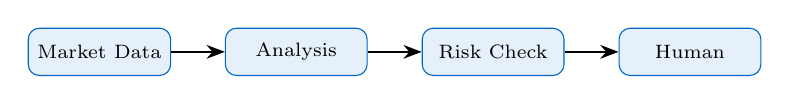
\begin{tikzpicture}[
    box/.style={rectangle, draw=arkblue, fill=arkblue!10, rounded corners, minimum width=1.8cm, minimum height=0.6cm, font=\scriptsize},
    arrow/.style={-{Stealth}, thick}
]
    \node[box] (data) at (0,0) {Market Data};
    \node[box] (analysis) at (2.5,0) {Analysis};
    \node[box] (risk) at (5,0) {Risk Check};
    \node[box] (human) at (7.5,0) {Human};

    \draw[arrow] (data) -- (analysis);
    \draw[arrow] (analysis) -- (risk);
    \draw[arrow] (risk) -- (human);
\end{tikzpicture}
\end{center}

\textbf{Note:} Human approval required for all trades.

% ==================== IMPLEMENTATION ====================
\section{Implementation}

\begin{center}
\footnotesize
\begin{tabular}{@{}ll@{}}
\toprule
\textbf{Component} & \textbf{Status} \\
\midrule
Module directory & \texttt{src/core/trading/} \\
Current state & Stub/framework \\
Data sources & (To be integrated) \\
Execution & (Manual only) \\
\bottomrule
\end{tabular}
\end{center}

\textbf{Current Status}: The trading module is a minimal stub. Full implementation requires:
\begin{itemize}
    \item Market data API integration
    \item Backtesting framework
    \item Paper trading validation
    \item Regulatory compliance review
\end{itemize}

% ==================== LIMITATIONS ====================
\section{Limitations}

\begin{itemize}
    \item \textbf{No backtesting}: No backtesting on historical data was performed. All examples are theoretical illustrations. This framework has not been validated against standard portfolio optimization (e.g., Markowitz mean-variance) or compared with established trading strategies.
    \item \textbf{No live validation}: The system has not been tested with real market data or real trades.
    \item \textbf{$\varphi$-allocation is heuristic}: The golden-ratio--based allocation is a design metaphor, not derived from financial theory.
\end{itemize}

% ==================== ETHICAL CONSIDERATIONS ====================
\section{Ethical Considerations}

\begin{itemize}
    \item \textbf{No manipulation}: System must not engage in market manipulation
    \item \textbf{Fair access}: Not designed for front-running or HFT
    \item \textbf{Transparency}: All logic explainable
    \item \textbf{Human oversight}: No autonomous trading
\end{itemize}

% ==================== CONCLUSION ====================
\section{Conclusion}

Trading Intelligence demonstrates how ARKHEION AGI capabilities can be applied to financial analysis. The system emphasizes \textbf{risk management}, \textbf{human oversight}, and \textbf{transparency} over aggressive automation.

\textbf{Future work}:
\begin{itemize}
    \item Sentiment analysis integration
    \item Multi-asset correlation modeling
    \item Explainable trade rationale
\end{itemize}

% ==================== REFERENCES ====================
\section*{References}

\begin{enumerate}
\footnotesize
    \item Markowitz, H. ``Portfolio Selection.'' Journal of Finance, 1952.
    \item Kelly, J.L. ``A New Interpretation of Information Rate.'' Bell System Technical Journal, 1956.
\end{enumerate}

\end{document}
